\documentclass[12pt,a4paper, twosite]{article}
\usepackage[utf8]{inputenc}
\usepackage[T1]{fontenc}
\usepackage{graphicx}
\usepackage{grffile}
\usepackage{longtable}
\usepackage{wrapfig}
\usepackage{rotating}
\usepackage[normalem]{ulem}
\usepackage{amsmath}
\usepackage{textcomp}
\usepackage{amssymb}
\usepackage{capt-of}
\usepackage{hyperref}
\usepackage[left=2.00cm, right=2.50cm, top=2.50cm, bottom=2.00cm]{geometry}
\usepackage{fancyhdr}
\usepackage[spanish]{babel}
\fancyhead[RO,LE]{\thepage}
\fancyhead[LO]{\emph{\uppercase{\leftmark}}}
\fancyfoot{}
\renewcommand{\headrulewidth}{1.0pt}
\pagestyle{fancy}
\date{\today}
\title{IEEE-830}
\hypersetup{
	pdfborder={0 0 0},
	pdfauthor={fasdas ads d},
	pdftitle={IEEE-830},
	pdfkeywords={hola},
	pdfsubject={hola mundo},
%	pdfcreator={Emacs 26.2 (Org mode 9.1.9)}, 
	pdflang={Spanish}}


\begin{document}
	\begin{titlepage}
		\maketitle
		
	\end{titlepage}

\section*{Historial de cambios  }
crear tabla de el versionado de los cambios 

\newpage
	\tableofcontents	
\newpage
	\section{Introducción}
	\label{sec:org60390fa}



	
	\subsection{Propósito}
	\label{sec:org434c3ef}
	Este documento presenta una especificación de requerimientos de software para unsistema de  posicionamiento de antena. Este dispositivo generalmente se conoce como rotador. 
	 
	Esta dirigido a técnicos, profesionales y operarios que intervengan en los sistemas de apuntamiento que posee el IAR.   

	
	
	\subsection{Ámbito del sistema}
	\label{sec:org12e44a1}
	Este sistema, se desarrolla como un subsistema del interferómetro MIA(https://www.iar.unlp.edu.ar/slider/observatorio/), y el proyecto de construcción de estaciones terrenas. Se utilizar para realizar el apuntamiento de radiofuentes, y el seguimiento de satelites en forma automática.  El nombre del sistema rotador sera ROT\_IAR. Adicionalmente, tiene espectativas de escalar, y realizar una producción en serie. 
	
	
	\subsection{Definiciones, Acrónimos y Abreviaturas}
	\label{sec:orgb158e36}
	
	ver los acrónimos al terminar el documento 
	
	
	\subsection{Referencias}
	\label{sec:org62711e0}
	ver tesis, y plan de trabajo ! 
	
	\subsection{Visión general del documento}
	\label{sec:orgdaca22c}
	
	Este documento se realiza siguiendo el estándar IEEE Std. 830-1998
	
	
	\section{Descripción general del documento}
	\label{sec:orgc1c4017}
	
	\subsection{Perspectiva del producto}
	\label{sec:org24980a8}
%	El proyecto aquí especificado es independiente de otros sistemas y no tiene relación con otros productos
	El software es parte de un sistema mayor, denominado interferómetro MIA y estaciones terrenas. Este sistema de apuntamiento, se adicionara al sistema mecánico de la antena que esta en fase de construcción. Este sistema, realizará el apuntamiento de antena, y este según el proyecto(MIA o estaciones terrenas) es automático o manual. El diagrama en bloques del sistema se muestra en la figura \ref{fig:diagramaBloques}. 
	
	 El presente documento describe los requerimientos de software del bloque single board computer, y las interfaces del sistema que se observa en la figura  \ref{fig:diagramaBloques}. 
	\begin{figure}[h!]
		\centering
		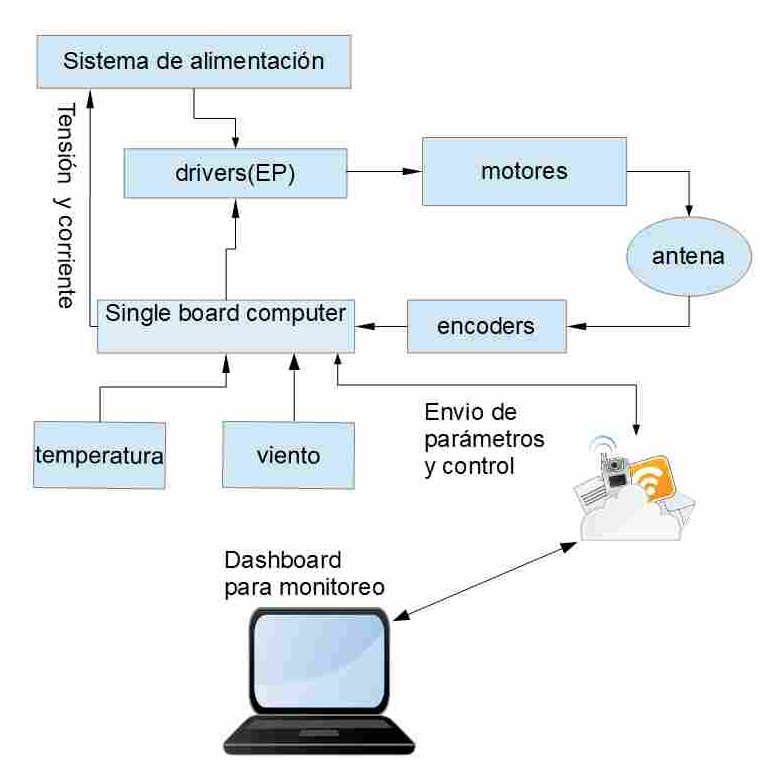
\includegraphics[scale=0.5]{bloquesInt.jpg}
		\caption{Diagrama en bloques del sistema}
		\label{fig:diagramaBloques}
	\end{figure}
	\subsection{Funciones del producto}
	\label{sec:orgaf51da6}
	\begin{enumerate}
		\item Servidor web embebido 
		\item Compatible con el software Gpredict y Stellarium, y scripts de antenas principales 
		\item Reinicio del en forma remota  
		\item Interrupción de operación en caso de condiciones climáticas adversas. 
		\item información de la operación y estado actual del sistema(tracking, untracked, y cenit). 
	\end{enumerate}
	
	\subsection{Características de los usuarios}
	\label{sec:orga40b0ee}
	Los usuarios serán técnicos, operarios y profesionales con conocimiento y experiencia en los sistemas de apuntamiento y manejo de rotadores. 
	\subsection{Restricciones}
	\label{sec:org5ca5790}
	
	
	\begin{itemize}
		
		\item Lenguaje python3 por cuestiones de compatibilidad de scripts de manejo principal de las antenas.
		\item El software debe estar bajo control de versiones.  
%		\item  se debe realizar un informe de avance por cada requerimiento que se cumple 
	\end{itemize}
	
	
	\subsection{Suposiciones y dependencias}
	\label{sec:org0ae23fe}
	
	
	
	\subsection{Requisitos futuros}
	\label{sec:org33cfcdb}
	Es deseable que el sistema posea control de velocidad. 
	
	
	
	\section{Requisitos específicos}
	\label{sec:org40573d1}
	
	Esta sección contiene los requisitos a un nivel de detalle suficiente
	como para permitir a los diseñadores diseñar un sistema que
	satisfaga estos requisitos, y demuestren si el sistema satisface, o
	no, los requisitos. Todo requisito aquí especificado describirá
	comportamientos externos del sistema, perceptibles por parte de los
	usuarios, operadores y otros sistemas. Esta es la sección más larga
	e importante de la ERS. Deberán aplicarse los siguientes principios:
	
	\begin{itemize}
		\item El documento debería ser perfectamente legible por personas de muy
		distintas formaciones e intereses.
		
		\item Deberán referenciarse aquellos documentos relevantes que poseen
		alguna influencia sobre los requisitos.
		
		\item Todo requisito deberá ser unívocamente identificable mediante algún
		código o sistema de numeración adecuado.
		
		\item Lo ideal, aunque en la práctica no siempre realizable, es que los
		requisitos posean las siguientes características: 
		
		\begin{itemize}
			\item \textbf{Corrección:} La ERS es correcta si y sólo si todo requisito que
			figura aquí(y que será implementado en el sistema) refleja alguna
			necesidad real. La corrección de la ERS implica que el sistema
			implementado será el deseado.
			
			\item \textbf{No ambiguos:} Cada requisito tiene una sola interpretación. Para
			eliminar la ambigüedad inherente a los requisitos expresados en
			lenguaje natural, se deberán utilizar gráficos o notaciones
			formales. En el caso de utilizar términos que, habitualmente,
			poseen más de una interpretación, se definirán con precisión en
			glosario.
			
			\item \textbf{Completos:} Todos los requisitos relevantes han sido incluidos en
			la ERS. Conviene incluir todas las posibles respuestas del sistema
			a los datos de entrada, tanto validos como no válidos.
			
			\item \textbf{Consistentes:} Los requisitos no pueden ser contradictorios. Un
			conjunto de requisitos contradictorios no es implementable.
			
			\item \textbf{Clasificados:} Normalmente, no todos los requisitos son igual de
			importantes. Los requisitos pueden clasificarse por importancia
			(esenciales, condicionales u opcionales) o por estabilidad (cambios
			que se espera que afecten al requisito). Esto sirve, ante todo,
			para no emplear excesivos recursos en implementar requisitos no
			esenciales.
			
			\item \textbf{Verificables:} La ERS es verificalble si y sólo si todos sus
			requisitos son verificables. Un requisito es verificable
			(testeable) si existe un proceso finito y no costoso para
			demostrar que el sistema cumple con el requisito. Un requisito
			ambiguo no es, en general, verificable. Expresiones como a veces,
			bien, adecuado, etc introducen ambigüedad en los
			requisitos. Requisitos como "en caso de accidente la nube tóxica
			no se extenderá más allá de 25km" no es verificable por el alto
			costo que conlleva.
			
			\item \textbf{Modificables:} La ERS es modificable si y sólo si se encuentra
			estructurada de forma que los cambios a los requisitos puedan
			realizarse de forma fácil, completa y consistente. La utilización
			de herramientas automáticas de gestión de requisito (por ejemplo
			RequisitePro o Doors) facilitan enormemente esta tarea.
			
			\item \textbf{Trazables:} La ERS es trazable si se conoce el origen de cada
			requisito y facilita la referencia de cada requisito a los
			componentes y de la implementación. La trazabilidad hacia atrás
			indica el origen (documento, persona, etc) de cada requisito. La
			trazabilidad hacia delante de un requisito R indica qué
			componentes del sistema son los que realizan el registro R.
		\end{itemize}
	\end{itemize}
	
	
	\subsection{Interfaces externas}
	\label{sec:orgfd5391f}
	
	Se describirán los requisitos que afecten a la interfaz de usuario,
	interfaz con otros sistemas (hardware y software) e interfaces de comunicaciones.
	
	
	\subsection{Funciones}
	\label{sec:org307bb59}
	
	Esta subsección (quizás la más larga del documento) deberá
	especificar todas aquellas acciones (funciones) que deberá llevar a
	cabo el software. Normalmente (aunque no siempre) son aquellas
	acciones expresables como "el sistema deberá \ldots{}" Si se considera
	necesario, podrán utilizarse notaciones gráficas y tablas, pero
	siempre supeditadas al lenguaje natural, y no al revés.
	
	Es importante tener en cuenta que, en 1983, el estándar de IEEE 830
	establecía que las funciones deberían expresarse como una jerarquía
	funcional (en paralelo con los DFDs propuestas por el análisis
	estructurado). Pero el estándar de IEEE 830, en sus últimas
	versiones, ya permite organizar esta subsección de múltiples formas,
	y sugiere, entre otras, las siguientes:
	
	
	\begin{itemize}
		\item Por tipos de usuarios: 
		Distintos usuarios poseen distintos requisitos. Para cada clase de
		usuario que exista en la organización, se especificarán los
		requisitos funcionales que le afecten o tengan mayor relación con
		sus tareas.
	\end{itemize}
	
	
	\begin{itemize}
		\item Por objetos:
		Los objetos son identidades del mundo real que serán reflejadas en
		el sistema. Para cada objeto, se detallarán sus atributos y sus
		funciones. Los objetos pueden agruparse en clases. Esta organización
		de la ERS no quiere decir que el diseño del sistema siga el
		paradigma de Orientación a Objetos.
	\end{itemize}
	
	
	\begin{itemize}
		\item Por estímulos: 
		Se especificarán los posibles estímulos que recibe el sistema y las
		funciones relacionadas con dicho estímulo.
	\end{itemize}
	
	
	\begin{itemize}
		\item Por jerarquía funcional: 
		Si ninguna de las anteriores alternativas resulta de ayuda, la
		funcionalidad del sistema se especificará como una jerarquía de
		funciones que comparten entradas, salidas o datos internos. Se
		detallarán las funciones (entrada, proceso, salida) y las
		subfunciones del sistema. Esto no implica que el diseño del sistema
		deba realizarse según el paradigma de diseño estructurado.
	\end{itemize}
	
	
	Para organizar esta subsección de la ERS se elegirá alguna de las
	anteriores alternativas, o incluso alguna otra que se considere más
	conveniente. Deberá, eso sí, justificarse el porqué de tal elección.
	
	
	
	\subsection{Requisitos de rendimiento}
	\label{sec:org94bc543}
	
	Se detallarán los requisitos relacionados con la carga que se espera
	tenga que soportar el sistema. Por ejemplo, el número de terminales,
	el número esperado de usuarios simultaneamente conectados, número de
	transacciones por segundo que deberá soportar el sistema, etc.
	También, si es necesario, se especificarpán los requisitos de
	datos, es decir, aquellos requisitos que afecten a la información
	que se guardará en la base de datos. Por ejemplo, la frecuencia de
	uso, las capacidades de acceso y la cantidad de registros que se
	espera almacenar (decenas, cientos, miles o millones).
	
	
	\subsection{Restricciones de diseño}
	\label{sec:org49fe900}
	
	
	Todo aquello que restrinja las decisiones relativas al diseño de la
	aplicación: Restricciones de otros estándares, limitaciones del
	hardware, etc.
	
	
	\subsection{Atributos del sistema}
	\label{sec:orgd0babc0}
	
	Se detallarán los atributos de calidad (las "ilities") del
	sistema. Fiablidad, manteniblidad, portabilidad, y muy importante,
	la seguridad. Deberá especificarse qué tipos de usuarios están
	autorizados, o no, a realizar ciertas tareas, y cómo se
	implementarán los mecanismos de seguridad (por ejemplo, por medio de
	un \emph{login} y una \emph{password}).
	
	
	\subsection{Otros requisitos}
	\label{sec:org31d2978}
	
	Cualquier otro requisito que no encaje en otra sección.
	
	\newpage
	
	
	\section{Apéndices}
	\label{sec:org75cea03}
	
	Puede contener todo tipo de información relevante para la ERS pero
	que, propiamente, no forme parte de la ERS. Por ejemplo:
	
	\begin{enumerate}
		\item Formatos de entrada/salida de datos, por pantalla o en listados.
		
		\item Resultados de análisis de costes.
		
		\item Restricciones acerca del lenguaje de programación.
	\end{enumerate}
\end{document}